\begin{frame}
  \frametitle{Porting the Linux kernel}
  \begin{itemize}
  \item The Linux kernel supports a lot of different CPU architectures
  \item Each of them is maintained by a different group of
    contributors
    \begin{itemize}
    \item See the \code{MAINTAINERS} file for details
    \end{itemize}
  \item The organization of the source code and the methods to port
    the Linux kernel to a new board are therefore very
    architecture-dependent
    \begin{itemize}
    \item For example, some architectures use the Device Tree, some do
      not.
    \end{itemize}
  \item This presentation is focused on the ARM architecture only
  \end{itemize}
\end{frame}

\begin{frame}
  \frametitle{Architecture, CPU and Machine}
  \begin{itemize}
  \item In the source tree, each architecture has its own directory
    \begin{itemize}
    \item \code{arch/arm} for the ARM architecture
    \end{itemize}
  \item This directory contains generic ARM code
    \begin{itemize}
    \item \code{boot}, \code{common}, \code{configs}, \code{kernel},
      \code{lib}, \code{mm}, \code{nwfpe}, \code{vfp},
      \code{oprofile}, \code{tools}
    \end{itemize}
  \item And many directories for different SoC families
    \begin{itemize}
    \item \code{mach-*} directories: \code{mach-pxa} for PXA CPUs,
      \code{mach-imx} for Freescale iMX CPUs, etc.
      \begin{itemize}
      \item Before the ARM cleanup, those directories contained
        support for the SoC family (GPIO, clocks, pinmux, power
        management, interrupt controller, etc.) and for the various
        boards.
      \item Nowadays, they contain a lot less code, essentially a
        small SoC description file, power management and SMP code.
      \end{itemize}
    \end{itemize}
  \item Some CPU types share some code, in directories named
    \code{plat-*}
  \item Device Tree files in \code{arch/arm/boot/dts}.
  \item Device drivers in \code{drivers/}.
  \end{itemize}
\end{frame}

\begin{frame}
  \frametitle{Before the Device Tree and ARM cleanup}
  \begin{itemize}
  \item Until 2011, the ARM architecture wasn't using the Device Tree,
    and a large portion of the SoC support was located in
    \code{arch/arm/mach-<foo>}.
  \item Each board supported by the kernel was associated to an unique
    {\em machine ID}.
  \item The entire list of {\em machine ID} can be downloaded at
    \url{http://www.arm.linux.org.uk/developer/machines/download.php}
    and one could freely register an additional one.
  \item The Linux kernel was defining a {\em machine structure} for
    each board, which associates the {\em machine ID} with a set of
    informations and callbacks.
  \item The bootloader had to pass the {\em machine ID} to the kernel
    in a specific ARM register.
  \end{itemize}
\end{frame}

\begin{frame}
  \frametitle{The Device Tree and the ARM cleanup}
  \begin{itemize}
  \item As the ARM architecture gained significantly in popularity,
    some major refactoring was needed.
  \item First, the Device Tree was introduced on ARM: instead of using
    C code to describe SoCs and boards, a specialized language is
    used.
  \item Second, many driver infrastructures were created to replace
    custom code in \code{arch/arm/mach-<foo>}:
    \begin{itemize}
    \item The common clock framework in \code{drivers/clk}
    \item The pinctrl subsystem in \code{drivers/pinctrl}
    \item The irqchip subsystem in \code{drivers/irqchip}
    \item The clocksource subsystem in \code{drivers/clocksource}
    \end{itemize}
  \item The amount of code in \code{mach-<foo>} has now significantly
    reduced.
  \end{itemize}
\end{frame}

\begin{frame}
  \frametitle{Adding the support for a new ARM board}
  Provided the SoC used on your board is supported by the Linux kernel:
  \begin{enumerate}
  \item Create a {\em Device Tree} file in \code{arch/arm/boot/dts},
    generally named \code{<soc-name>-<board-name>.dts}, and make it
    include the relevant SoC \code{.dtsi} file.
    \begin{itemize}
    \item Your Device Tree will describe all the SoC peripherals that
      are enabled, the pin muxing, as well as all the devices on the
      board.
    \end{itemize}
  \item Modify \code{arch/arm/boot/dts/Makefile} to make sure your
    Device Tree gets built as a {\em DTB} during the kernel build.
  \item If needed, develop the missing device drivers for the devices
    that are on your board outside the SoC.
  \end{enumerate}
\end{frame}

\begin{frame}
  \frametitle{Example of the Marvell Armada 370/XP SoCs}
  \begin{itemize}
  \item The hardware platform used in this training is based on the
    AM335x processor from Texas Instruments.
  \item This platform inherits from the OMAP family of TI, for which
    kernel support has been around for a long time.
  \item Due to this, and the complexity of the platform, the AM335x
    and OMAP support in the kernel hasn't fully migrated yet to all
    the infrastructures created during the {\em ARM cleanup}.
  \item Therefore, to illustrate this section, we will take the
    example of the Marvell Armada 370/XP platform, on which Free
    Electrons has worked specifically.
  \end{itemize}
\end{frame}

\begin{frame}
  \frametitle{Studying the OpenBlocks AX3-4 platform}
  \begin{columns}
    \column{0.7\textwidth}
    \begin{itemize}
    \item OpenBlocks AX3-4
    \item Uses the dual-core Marvell Armada MV78260, from the Armada
      XP family.
    \item 1 GB of RAM
    \item 4 Gigabit Ethernet ports
    \item 2 serial ports, one button, 3 LEDS
    \item Two I2Cs bus, one equipped with a RTC
    \item Two SATA ports, one internal, one external
    \item Two USB ports
    \item One mini-PCIe connector
    \item One 128 MB NOR flash
    \end{itemize}
    \column{0.3\textwidth}
    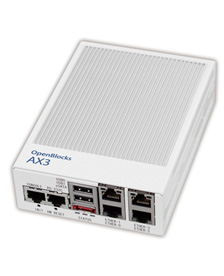
\includegraphics[width=\textwidth]{slides/kernel-porting-content/openblocks.jpg}
  \end{columns}
\end{frame}

\begin{frame}[fragile]
  \frametitle{OpenBlocks AX3-4 Device Tree, 1}
  \begin{itemize}
  \item Mandatory Device Tree language definition\\
    \mint[fontsize=\footnotesize]{perl}+/dts-v1+
  \item Include the \code{.dtsi} file describing the SoC\\
    \mint[fontsize=\footnotesize]{perl}+#include "armada-xp-mv78260.dtsi"+
  \item Start the root of the tree\\
    \mint[fontsize=\footnotesize]{perl}+/ {+
  \item A human-readable string to describe the machine\\
    \mint[fontsize=\footnotesize]{perl}+  model = "PlatHome OpenBlocks AX3-4 board";+
  \item A list of {\em compatible} strings, from the most specific one
    to the most general one. Can be used by kernel code to do a SoC or
    board-specific check. Currently only used to find the
    corresponding SoC support\\
    \scriptsize
    \begin{minted}[fontsize=\footnotesize]{perl}
    compatible = "plathome,openblocks-ax3-4",
        "marvell,armadaxp-mv78260", "marvell,armadaxp",
        "marvell,armada-370-xp";
      \end{minted}
  \end{itemize}
\end{frame}

\begin{frame}[fragile]
  \frametitle{OpenBlocks AX3-4 Device Tree, 1}
  \begin{itemize}
  \item Definition of the default {\em kernel command line}. Some
    additional operating-system specific entries can be added in
    \code{chosen}:
    \begin{minted}[fontsize=\footnotesize]{perl}
chosen {
        bootargs = "console=ttyS0,115200 earlyprintk";
};
\end{minted}
\item Definition of the size and location of the RAM:
    \begin{minted}[fontsize=\footnotesize]{perl}
memory {
        device_type = "memory";
        reg = <0 0x00000000 0 0xC0000000>; /* 3 GB */
};
      \end{minted}
  \end{itemize}
\end{frame}